\documentclass{anstrans}
%%%%%%%%%%%%%%%%%%%%%%%%%%%%%%%%%%%
\title{Pyre: A Cyclus Pyroprocessing Facility Archetype}
\author{Gregory T. Westphal$^*$ and Kathryn D. Huff}

\institute{
Dept. of Nuclear, Plasma and Radiological Engineering, University of Illinois at Urbana-Champaign \\
$^*$gtw2@illinois.edu
}

%%%% packages and definitions (optional)
\usepackage{float}
\floatstyle{plaintop}
\restylefloat{table}
\usepackage{graphicx} % allows inclusion of graphics
\usepackage{booktabs} % nice rules (thick lines) for tables
\usepackage{microtype} % improves typography for PDF
\usepackage{xspace}
\usepackage{tabularx}
\newcommand{\SN}{S$_N$}
\renewcommand{\vec}[1]{\bm{#1}} %vector is bold italic
\newcommand{\vd}{\bm{\cdot}} % slightly bold vector dot
\newcommand{\grad}{\vec{\nabla}} % gradient
\newcommand{\ud}{\mathop{}\!\mathrm{d}} % upright derivative symbol
\newcommand{\Cyclus}{\textsc{Cyclus}\xspace}%
\newcommand{\Cycamore}{\textsc{Cycamore}\xspace}%
\newcolumntype{c}{>{\hsize=.56\hsize}X}
\newcolumntype{b}{>{\hsize=.7\hsize}X}
\newcolumntype{s}{>{\hsize=.74\hsize}X}
\newcolumntype{f}{>{\hsize=.1\hsize}X}
\newcolumntype{a}{>{\hsize=.45\hsize}X}

\usepackage{amsmath}

\usepackage[acronym,toc]{glossaries}
%\newacronym{<++>}{<++>}{<++>}
\newacronym[longplural={metric tons of heavy metal}]{MTHM}{MTHM}{metric ton of heavy metal}
\newacronym[longplural={metric tons of initial heavy metal}]{MTIHM}{MTIHM}{metric ton of initial heavy metal}
\newacronym{ABM}{ABM}{agent-based modeling}
\newacronym{ACDIS}{ACDIS}{Program in Arms Control \& Domestic and International Security}
\newacronym{AHTR}{AHTR}{Advanced High Temperature Reactor}
\newacronym{ANDRA}{ANDRA}{Agence Nationale pour la gestion des D\'echets RAdioactifs, the French National Agency for Radioactive Waste Management}
\newacronym{ANL}{ANL}{Argonne National Laboratory}
\newacronym{API}{API}{application programming interface}
\newacronym{ARCH}{ARCH}{autoregressive conditional heteroskedastic}
\newacronym{ARE}{ARE}{Aircraft Reactor Experiment}
\newacronym{ARFC}{ARFC}{Advanced Reactors and Fuel Cycles}
\newacronym{ARMA}{ARMA}{autoregressive moving average}
\newacronym{ASME}{ASME}{American Society of Mechanical Engineers}
\newacronym{ATWS}{ATWS}{Anticipated Transient Without Scram}
\newacronym{BDBE}{BDBE}{Beyond Design Basis Event}
\newacronym{BIDS}{BIDS}{Berkeley Institute for Data Science}
\newacronym{BOL}{BOL}{Beginning-of-Life}
\newacronym{BSD}{BSD}{Berkeley Software Distribution}
\newacronym{CAFCA}{CAFCA}{ Code for Advanced Fuel Cycles Assessment }
\newacronym{CASL}{CASL}{Consortium for Advanced Simulation of Light Water Reactors}
\newacronym{CDTN}{CDTN}{Centro de Desenvolvimento da Tecnologia Nuclear}
\newacronym{CEA}{CEA}{Commissariat \`a l'\'Energie Atomique et aux \'Energies Alternatives}
\newacronym{CI}{CI}{continuous integration}
\newacronym{CNEC}{CNEC}{Consortium for Nonproliferation Enabling Capabilities}
\newacronym{CNEN}{CNEN}{Comiss\~{a}o Nacional de Energia Nuclear}
\newacronym{CNERG}{CNERG}{Computational Nuclear Engineering Research Group}
\newacronym{COSI}{COSI}{Commelini-Sicard}
\newacronym{COTS}{COTS}{commercial, off-the-shelf}
\newacronym{CSNF}{CSNF}{commercial spent nuclear fuel}
\newacronym{CTAH}{CTAHs}{Coiled Tube Air Heaters}
\newacronym{CUBIT}{CUBIT}{CUBIT Geometry and Mesh Generation Toolkit}
\newacronym{CURIE}{CURIE}{Centralized Used Fuel Resource for Information Exchange}
\newacronym{DAG}{DAG}{directed acyclic graph}
\newacronym{DANESS}{DANESS}{Dynamic Analysis of Nuclear Energy System Strategies}
\newacronym{DBE}{DBE}{Design Basis Event}
\newacronym{DESAE}{DESAE}{Dynamic Analysis of Nuclear Energy Systems Strategies}
\newacronym{DHS}{DHS}{Department of Homeland Security}
\newacronym{DOE}{DOE}{Department of Energy}
\newacronym{DRACS}{DRACS}{Direct Reactor Auxiliary Cooling System}
\newacronym{DRE}{DRE}{dynamic resource exchange}
\newacronym{DSNF}{DSNF}{DOE spent nuclear fuel}
\newacronym{DYMOND}{DYMOND}{Dynamic Model of Nuclear Development }
\newacronym{EBS}{EBS}{Engineered Barrier System}
\newacronym{EDZ}{EDZ}{Excavation Disturbed Zone}
\newacronym{EIA}{EIA}{U.S. Energy Information Administration}
\newacronym{EPA}{EPA}{Environmental Protection Agency}
\newacronym{EP}{EP}{Engineering Physics}
\newacronym{FCO}{FCO}{Fuel Cycle Options}
\newacronym{FCT}{FCT}{Fuel Cycle Technology}
\newacronym{FCWMD}{FCWMD}{Fuel Cycle and Waste Management Division}
\newacronym{FEHM}{FEHM}{Finite Element Heat and Mass Transfer}
\newacronym{FEPs}{FEPs}{Features, Events, and Processes}
\newacronym{FHR}{FHR}{Fluoride-Salt-Cooled High-Temperature Reactor}
\newacronym{FLiBe}{FLiBe}{Fluoride-Lithium-Beryllium}
\newacronym{GCAM}{GCAM}{Global Change Assessment Model}
\newacronym{GDSE}{GDSE}{Generic Disposal System Environment}
\newacronym{GDSM}{GDSM}{Generic Disposal System Model}
\newacronym{GENIUSv1}{GENIUSv1}{Global Evaluation of Nuclear Infrastructure Utilization Scenarios, Version 1}
\newacronym{GENIUSv2}{GENIUSv2}{Global Evaluation of Nuclear Infrastructure Utilization Scenarios, Version 2}
\newacronym{GENIUS}{GENIUS}{Global Evaluation of Nuclear Infrastructure Utilization Scenarios}
\newacronym{GPAM}{GPAM}{Generic Performance Assessment Model}
\newacronym{GRSAC}{GRSAC}{Graphite Reactor Severe Accident Code}
\newacronym{GUI}{GUI}{graphical user interface}
\newacronym{GWd}{GWd}{Gigawatt Days}
\newacronym{HLW}{HLW}{high level waste}
\newacronym{HPC}{HPC}{high-performance computing}
\newacronym{HTC}{HTC}{high-throughput computing}
\newacronym{HTGR}{HTGR}{High Temperature Gas-Cooled Reactor}
\newacronym{IAEA}{IAEA}{International Atomic Energy Agency}
\newacronym{IEMA}{IEMA}{Illinois Emergency Mangament Agency}
\newacronym{INL}{INL}{Idaho National Laboratory}
\newacronym{IPRR1}{IRP-R1}{Instituto de Pesquisas Radioativas Reator 1}
\newacronym{IRP}{IRP}{Integrated Research Project}
\newacronym{ISFSI}{ISFSI}{Independent Spent Fuel Storage Installation}
\newacronym{ISRG}{ISRG}{Independent Student Research Group}
\newacronym{JFNK}{JFNK}{Jacobian-Free Newton Krylov}
\newacronym{KAERI}{KAERI}{Korea Atomic Energy Research Institute}
\newacronym{LANL}{LANL}{Los Alamos National Laboratory}
\newacronym{LBNL}{LBNL}{Lawrence Berkeley National Laboratory}
\newacronym{LCOE}{LCOE}{levelized cost of electricity}
\newacronym{LDRD}{LDRD}{laboratory directed research and development}
\newacronym{LFR}{LFR}{Lead-Cooled Fast Reactor}
\newacronym{LGPL}{LGPL}{Lesser GNU Public License}
\newacronym{LLNL}{LLNL}{Lawrence Livermore National Laboratory}
\newacronym{LMFBR}{LMFBR}{Liquid-Metal-cooled Fast Breeder Reactor}
\newacronym{LOFC}{LOFC}{Loss of Forced Cooling}
\newacronym{LOHS}{LOHS}{Loss of Heat Sink}
\newacronym{LOLA}{LOLA}{Loss of Large Area}
\newacronym{LP}{LP}{linear program}
\newacronym{LWR}{LWR}{Light Water Reactor}
\newacronym{MARKAL}{MARKAL}{MARKet and ALlocation}
\newacronym{MA}{MA}{minor actinide}
\newacronym{MCNP}{MCNP}{Monte Carlo N-Particle code}
\newacronym{MILP}{MILP}{mixed-integer linear program}
\newacronym{MIT}{MIT}{the Massachusetts Institute of Technology}
\newacronym{MOAB}{MOAB}{Mesh-Oriented datABase}
\newacronym{MOOSE}{MOOSE}{Multiphysics Object-Oriented Simulation Environment}
\newacronym{MOX}{MOX}{mixed oxide}
\newacronym{MSBR}{MSBR}{Molten Salt Breeder Reactor}
\newacronym{MSRE}{MSRE}{Molten Salt Reactor Experiment}
\newacronym{MSR}{MSR}{Molten Salt Reactor}
\newacronym{MWd}{MWd}{Megawatt Days}
\newacronym{NAGRA}{NAGRA}{National Cooperative for the Disposal of Radioactive Waste}
\newacronym{NCSA}{NCSA}{National Center for Supercomputing Applications}
\newacronym{NEAMS}{NEAMS}{Nuclear Engineering Advanced Modeling and Simulation}
\newacronym{NEUP}{NEUP}{Nuclear Energy University Programs}
\newacronym{NFCSim}{NFCSim}{Nuclear Fuel Cycle Simulator}
\newacronym{NFC}{NFC}{Nuclear Fuel Cycle}
\newacronym{NGNP}{NGNP}{Next Generation Nuclear Plant}
\newacronym{NMWPC}{NMWPC}{Nuclear MW Per Capita}
\newacronym{NNSA}{NNSA}{National Nuclear Security Administration}
\newacronym{NPRE}{NPRE}{Department of Nuclear, Plasma, and Radiological Engineering}
\newacronym{NQA1}{NQA-1}{Nuclear Quality Assurance - 1}
\newacronym{NRC}{NRC}{Nuclear Regulatory Commission}
\newacronym{NSF}{NSF}{National Science Foundation}
\newacronym{NSSC}{NSSC}{Nuclear Science and Security Consortium}
\newacronym{NUWASTE}{NUWASTE}{Nuclear Waste Assessment System for Technical Evaluation}
\newacronym{NWF}{NWF}{Nuclear Waste Fund}
\newacronym{NWTRB}{NWTRB}{Nuclear Waste Technical Review Board}
\newacronym{OCRWM}{OCRWM}{Office of Civilian Radioactive Waste Management}
\newacronym{ORION}{ORION}{ORION}
\newacronym{ORNL}{ORNL}{Oak Ridge National Laboratory}
\newacronym{PARCS}{PARCS}{Purdue Advanced Reactor Core Simulator}
\newacronym{PBAHTR}{PB-AHTR}{Pebble Bed Advanced High Temperature Reactor}
\newacronym{PBFHR}{PB-FHR}{Pebble-Bed Fluoride-Salt-Cooled High-Temperature Reactor}
\newacronym{PEI}{PEI}{Peak Environmental Impact}
\newacronym{PH}{PRONGHORN}{PRONGHORN}
\newacronym{PI}{PI}{Principal Investigator}
\newacronym{PNNL}{PNNL}{Pacific Northwest National Laboratory}
\newacronym{PRIDE}{PRIDE}{Pyroprocessing Integrated Demonstration}
\newacronym{PRKE}{PRKE}{Point Reactor Kinetics Equations}
\newacronym{PSPG}{PSPG}{Pressure-Stabilizing/Petrov-Galerkin}
\newacronym{PWAR}{PWAR}{Pratt and Whitney Aircraft Reactor}
\newacronym{PWR}{PWR}{Pressurized Water Reactor}
\newacronym{PyNE}{PyNE}{Python toolkit for Nuclear Engineering}
\newacronym{PyRe}{PyRe}{Pyro Reprocessing Module}
\newacronym{PyRK}{PyRK}{Python for Reactor Kinetics}
\newacronym{QA}{QA}{quality assurance}
\newacronym{RDD}{RD\&D}{Research Development and Demonstration}
\newacronym{RD}{R\&D}{Research and Development}
\newacronym{RELAP}{RELAP}{Reactor Excursion and Leak Analysis Program}
\newacronym{RIA}{RIA}{Reactivity Insertion Accident}
\newacronym{RIF}{RIF}{Region-Institution-Facility}
\newacronym{SAM}{SAM}{Simulation and Modeling}
\newacronym{SCF}{SCF}{Software Carpentry Foundation}
\newacronym{SFR}{SFR}{Sodium-Cooled Fast Reactor}
\newacronym{SINDAG}{SINDA{\textbackslash}G}{Systems Improved Numerical Differencing Analyzer $\backslash$ Gaski}
\newacronym{SKB}{SKB}{Svensk K\"{a}rnbr\"{a}nslehantering AB}
\newacronym{SNF}{SNF}{spent nuclear fuel}
\newacronym{SNL}{SNL}{Sandia National Laboratory}
\newacronym{SNM}{SNM}{Special Nuclear Material}
\newacronym{STC}{STC}{specific temperature change}
\newacronym{SUPG}{SUPG}{Streamline-Upwind/Petrov-Galerkin}
\newacronym{SWF}{SWF}{Separations and Waste Forms}
\newacronym{SWU}{SWU}{Separative Work Unit}
\newacronym{SandO}{S\&O}{Signatures and Observables}
\newacronym{THW}{THW}{The Hacker Within}
\newacronym{TRIGA}{TRIGA}{Training Research Isotope General Atomic}
\newacronym{TRISO}{TRISO}{Tristructural Isotropic}
\newacronym{TRU}{TRU}{transuranic} 
\newacronym{TSM}{TSM}{Total System Model}
\newacronym{TSPA}{TSPA}{Total System Performance Assessment for the Yucca Mountain License Application}
\newacronym{UFD}{UFD}{Used Fuel Disposition}
\newacronym{UML}{UML}{Unified Modeling Language}
\newacronym{UOX}{UOX}{uranium oxide}
\newacronym{UQ}{UQ}{uncertainty quantification}
\newacronym{US}{US}{United States}
\newacronym{UW}{UW}{University of Wisconsin}
\newacronym{VISION}{VISION}{the Verifiable Fuel Cycle Simulation Model}
\newacronym{VV}{V\&V}{verification and validation}
\newacronym{WIPP}{WIPP}{Waste Isolation Pilot Plant}
\newacronym{YMG}{YMG}{Young Members Group}
\newacronym{YMR}{YMR}{Yucca Mountain Repository Site}

\makeglossaries

\begin{document}
%%%%%%%%%%%%%%%%%%%%%%%%%%%%%%%%%%%%%%%%%%%%%%%%%%%%%%%%%%%%%%%%%%%%%%%%%%%%%%%%
\begin{abstract}
Quantifying potential signatures and observables of material diverted from a 
pyroprocessing facility presents a modeling challenge.
This work assesses system parameters that influence separation efficiency and 
throughput. We leverage these parameters to implement a customizable pyroprocessing facility \emph{archetype}, Pyre, for use with the Cyclus framework.
This generic facility model will allow simulations to 
quantify signatures and observables associated with various operational modes 
and material throughputs for a variety of facility designs. Such quantification 
can aid timely detection of material diversion. 
This paper describes the Pyre facility archetype design, pyroprocessing flowsheets captured by the model, and simulation capabilities it enables. 
To analyze data retrieved from the model, we additionally propose a class for tracking and 
observing signatures and observables which will be extensible for other 
facility archetypes in the future.
\end{abstract}
\section{Introduction}
The diversion of significant quantities of SNM from the nuclear fuel cycle is major non-proliferation 
concern \cite{noauthor_iaea_2017}. These diversions must be detected in a timely manner using signatures and observables in 
order to properly safegaurd the fuel cycle. Timely detection is critical in non-proliferation to discover these shadow fuel cycles
before diverted material is further processed. Pyroprocessing is a used nuclear fuel separations technology for advanced reactors. 
With a reprocessing technology comes signatures and observables which in turn necessitate unique diversion detection methods. 
The goal of this research is to identify potential signs of material diversion in a pyroprocessing facility and implement models 
of these processes into a detailed pyroprocessing facility archetype to the modular, agent-based, fuel cycle simulator, \Cyclus \cite{huff_fundamental_2016}. This facility archetype will equip users of the \Cyclus fuel cycle simulator to investigate the 
detection timeliness enabled by measuring signatures and observables in various fuel cycle scenarios.
%%%%%%%%%%%%%%%%%%%%%%%%%%%%%%%%%%%%%%%%%%%%%%%%%%%%%%%%%%%%%%%%%%%%%%%%%%%%%%%%
\section{Background: \Cyclus}
\Cyclus models the flow of material through user-defined nuclear fuel cycle scenarios. Facilities in nuclear fuel cycles vary, 
requiring a diverse collection of pre-designed facility process models, known as \emph{archetypes}. \Cycamore, the CYClus 
Additional MOdules REpository, provides common facility archetypes (separations, enrichment, reactor, etc.)
\cite{carlsen_cycamore_2014}. Archetypes are customizable agent models which populate the simulation. Simulations run in discrete time steps and allow exact isotopes to be dynamically tracked between facilities \cite{huff_fundamental_2016}. This work seeks to add signature and observable tacking capabilities to \Cyclus. Potentially trackable signatures and observables include truck deliveries, power draw, and steam production  \cite{Hou_2016,Yilmaz_2016}. This list is expanded upon in Table \ref{tab:params} to include pyroprocessing parameters.
\Cyclus' discrete time allows users to investigate diversion and flag the time and location diversion occurs.

%%%%%%%%%%%%%%%%%%%%%%%%%%%%%%%%%%%%%%%%%%%%%%%%%%%%%%%%%%%%%%%%%%%%%%%%%%%%%%%%
\section{Pyroprocessing}
Pyroprocessing is an electrochemical separation process used to recycle spent fuel into metallic fuel for use in advanced reactors.
Separation efficiencies will differ according to design and fuel type. There are four major 
systems within pyroprocessing with observable waste: voloxidation, electroreduction, electrorefining, and electrowinning \cite{Borrelli_2017}.  

\begin{figure}[ht] % replace 't' with 'b' to force it to be on the bottom
	\centering
	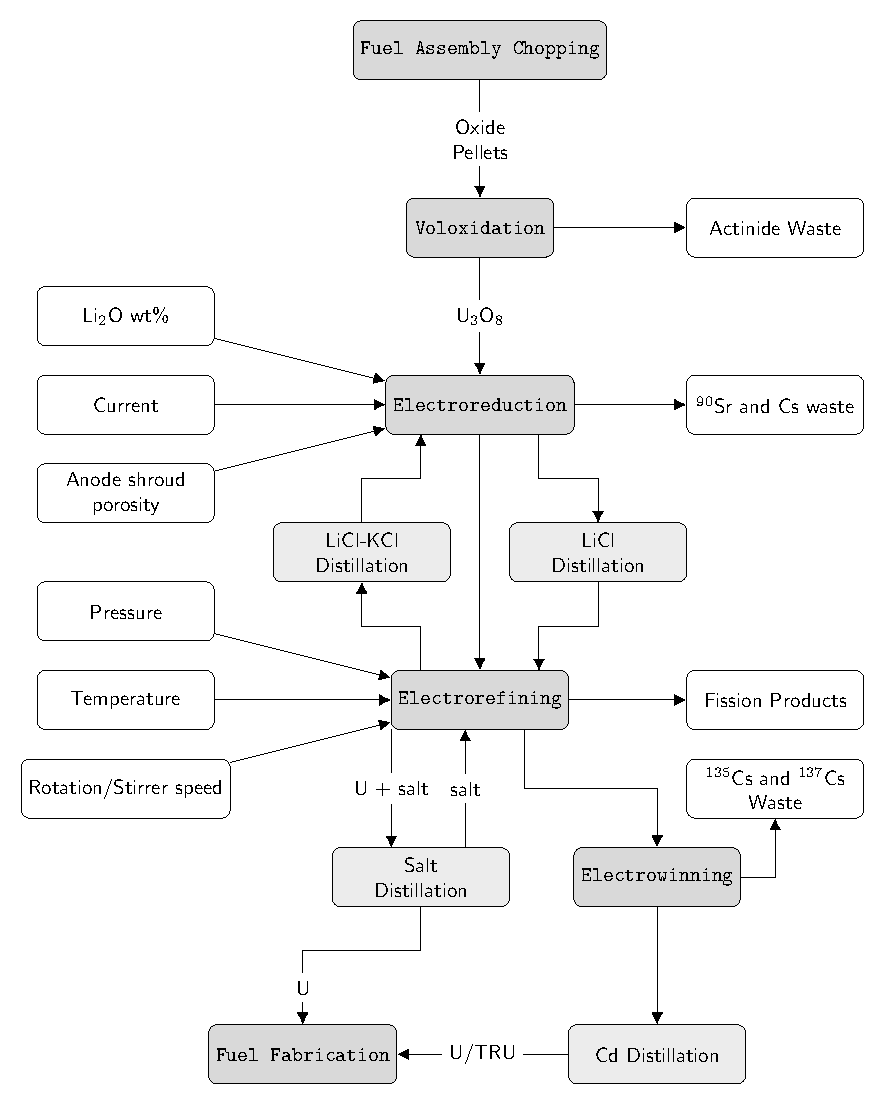
\includegraphics[width=0.5\textwidth]{flowchart}
	\caption{An archetype design flowchart of pyroprocessing facilities including observable outputs and \Cyclus variables.}
	\label{fig:flowchart}
\end{figure}

Figure \ref{fig:flowchart} demonstrates the primary separations steps involved in a general pyroprocessing facility. The main process 
parameters are along the left side of the flowsheet, each applied to processes most significantly impacted. The boxes on the 
right side of the processes contain the observable waste produced by each step that \Cyclus can track. Each of the main processes 
are described below regarding information to be used by \Cyclus.

\subsection{Voloxidation}

LWR fuel must be treated and separated before proceeding with electrolytic processes. Heated under 
500$^{\circ}$C, noble gases, carbon, and tritium are collected to decay in storage, and uranium dioxide is converted to $U_3O_8$. 
Actinides are also converted to their stable oxide forms and a majority are removed \cite{flowsheet_1998,jubin_spent_2009}. 
Voloxidation throughput can be increased by heating the uranium dioxide to temperatures in excess of 800$^{\circ}$C. 
Other methods to improve the U$_3$O$_8$ reaction rate are to use alternative oxidants such as cycling between H$_2$ and air \cite{jubin_spent_2009}.

\begin{figure}[ht]
	\centering
	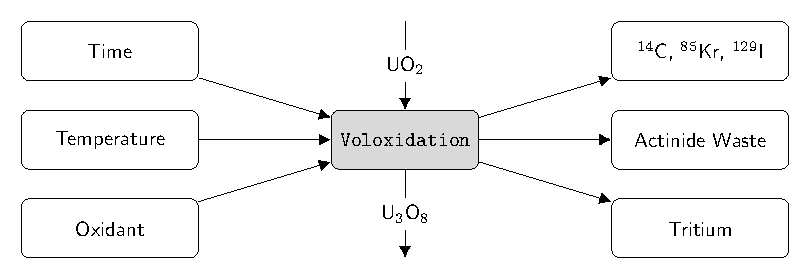
\includegraphics[width=1\linewidth]{volox}
	\caption{A material balance over the voloxidation sub-process, including observables.}
	\label{fig:volox}
\end{figure}

\subsection{Electroreduction}

Yellowcake, created in voloxidation, enters the cathode, a negatively charged metal basket. A Current density between 100 and 
500 mA/cm$^2$ 
is applied to the anode in a molten LiCl salt. The electrolytic reduction process primarily results in the diffusion of 
Cs, Ba and Sr, along with the reduction and conversion of zirconium into metallic form \cite{choi_electrochemical_2015,flowsheet_1998}.
Electroreduction can further improve its throughput by the addition of Li$_2$O as a catalyst; the catalyst also prevents dissolution 
of the anode \cite{choi_electrochemical_2015}. Since Li$_2$O is used to speed up the reaction, note 
that for signatures and observables the operators could add more oxide than reported to IAEA. More frequent shipments 
of lithium oxide can be tracked as an observable to match records.

\begin{figure}[ht]
	\centering
	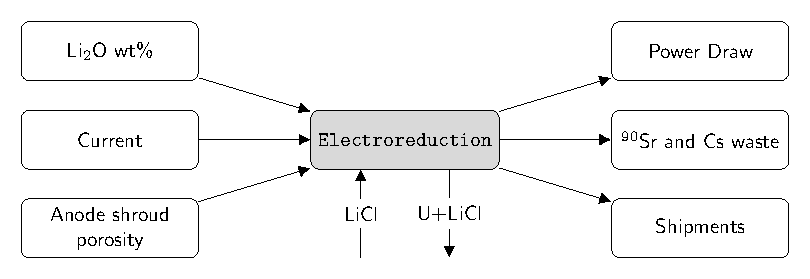
\includegraphics[width=1\linewidth]{reduction}
	\caption{A material balance over the electroreduction process with signatures and observables.}
	\label{fig:reduction}
\end{figure}

Electroreduction produces the majority of Sr and Cs waste compared to electrowinning. This stream has considerable decay 
signature proportional to the efficiency and size of the feed batch \cite{Borrelli_2017,flowsheet_1998}.

\subsection{Electrorefining}

The uranium and salt mixture from reduction is fed into an anode basket suspended in a graphite cathode. A LiCl-KCl eutectic is used as 
an electrolyte above 500$^{\circ}$C \cite{flowsheet_1998,lee_korean_2011}. The uranium dissolves at the anode to recombine at 
the cathode as metallic uranium. The waste transuranics (TRUs) and lathanides are in a soluble chloride form  while fission 
products and cladding remain in the anode basket. Finally, actinides and fission products are removed from the cladding 
electrochemically \cite{lee_korean_2011}.

Lee et al. \cite{lee_advanced_2008} show that the addition of vacuum pressure to the system improves removal efficiency. 
Temperature, however, exhibits the opposite effect: as temperature decreases so does salt removal. This comes into effect 
particularly depending on material choice of instrumentation and containment \cite{lee_advanced_2008}. The most limiting 
material choice is iron because a eutectic forms between Fe and U at 725$^{\circ}$C \cite{chapman_revision_1984}. 
In facilities where iron equipment is present temperatures are limited to 700$^{\circ}$C, and efficiency is 
significantly hindered. Cathode arrangement and anode rotation speed also affect the collection of uranium 
dendrites \cite{lee_advanced_2008}. The addition of a central stirrer allows mixing of uranium dendrites stuck on 
the bottom of the vessel, improving separation efficiency and increasing throughput. 

\begin{figure}[ht]
	\centering
	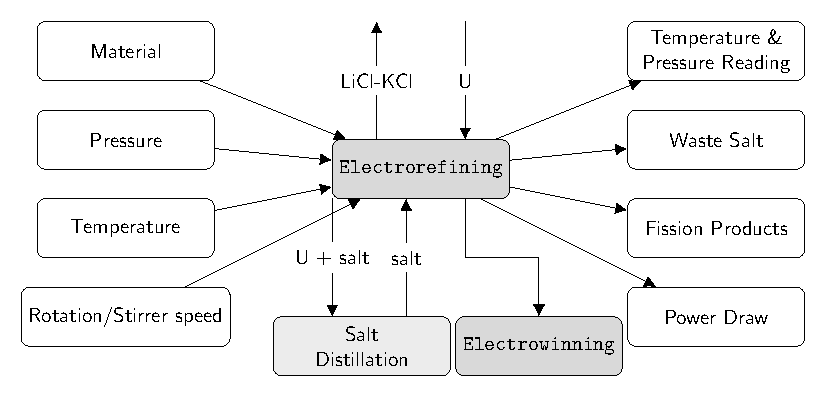
\includegraphics[width=0.9\linewidth]{refining}
	\caption{A material balance over the electrorefining sub-process, including observables.}
	\label{fig:refining}
\end{figure}

The electrorefining process also produces the fission product waste stream which requires monitoring. The following products are produced 
and tracked in this step: Tc, Ag, Pd, Rh, Ru, Mo and Zr \cite{flowsheet_1998}.

\subsection{Electrowinning}

The molten salt contains TRUs from electrorefining that are separated through electrowinning with trace uranium quantities. 
With a temperature of 500$^{\circ}$C there is approximately 99 wt\% reduction in actinides and lanthanides \cite{flowsheet_1998}. 
Throughput is also dependent on material choice for the inert electrodes whose operating voltages vary, impacting separation 
efficiency \cite{koyama_development_2012}. A shroud surrounds the anode to provide a path for O$^{2-}$ ions to the anode and 
prevent Cl$_2$ from corroding the anode \cite{kim_development_2013,choi_electrochemical_2015}. Optimum operating current 
depends on the material choice for the anode shroud since a nonporous shroud limits ion pathways to the points of contact 
with the anode. Higher porosity corresponds to free ion paths and a higher current. With a higher current, the separation 
time for electroreduction and electrowinning are reduced \cite{choi_electrochemical_2015}.

\begin{figure}[ht]
	\centering
	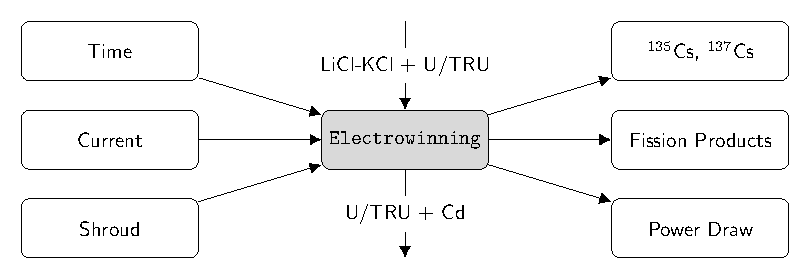
\includegraphics[width=1\linewidth]{winning}
	\caption{A material balance over the electrowinning sub-process, including observables.}
	\label{fig:winning}
\end{figure}

Figure \ref{fig:winning} shows that electrowinning produces Cs waste similar to electroreduction except in reduced quantities. Any fission products remaining in the salt from electrorefining are also removed here. In addition to physically tracked quantities, facility power can also be monitored to observe the use of current to increase throughput. 
%%%%%%%%%%%%%%%%%%%%%%%%%%%%%%%%%%%%%%%%%%%%%%%%%%%%%%%%%%%%%%%%%%%%%%%%%%%%%%%%
\section{Method: \Cyclus Simulation}
The separations facility provided by the \Cycamore library is used as an 
initial model of a simple \gls{PRIDE} facility. 
The user provides the separations archetype with a feed stream and facility efficiencies.  
Each waste stream requires a material balance over voloxidation, electroreduction, electrorefining and electrowinning. The main 
waste streams are metallic waste, ceramic waste from electrowinning and electroreduction, and vitrified waste. Vitrified 
waste contains the majority of TRUs, Sr, and rare-earth elements. The elemental separation efficiencies are 
determined through theoretical material balance determined by the NEA and Hermann et al \cite{flowsheet_1998,herrmann_separation_2010}. 
The simple simulation using a separations facility was run to verify the table of efficiencies input to \Cyclus. A scenario was 
created of one separations facility with a feed of five year cooled spent LWR 
fuel at a burn-up of 45 \gls{GWd} per \gls{MTIHM} to 
match results seen in \cite{flowsheet_1998}.

A pyroprocessing facility can be modeled with the separations archetype at low fidelity 
by a dedicated archetype. The goal for Pyre is to include facility configuration parameters and 
their respective effects on the efficiency table. Efficiencies also vary according to the feed stream resulting in different 
waste streams for LWR and FR fuels, for example. Multiple material choices exist for anodes and cathodes as well as other 
design choices that require consideration. 

\subsection{Parameters}
Facility configuration parameters customize the pyroprocessing archetype. Facility designs vary in 
multiple aspects which affect the throughput and efficiencies of different waste streams. Variables have been described above through material balance of each sub-process and their system parameters. Table \ref{tab:params} consists of the  derived from the previously mentioned process parameters and material flow. 

\begin{table}[h]
	\centering
	\begin{tabularx}{0.5\textwidth}{llcr}
		\hline
		\textbf{Sub-process} & \textbf{Parameters} & \textbf{S \& O} & \textbf{Refs} \\
		\hline
		Voloxidation & Volume & Tritium & \cite{jubin_spent_2009} \\
		& Oxidant & $^{14}$C & \cite{flowsheet_1998} \\
		& Flow Rate &  $^{129}$I &  \\
		& Temperature & $^{85}$Kr &  \\
		& Time & Actinides & \\ \hline
		Electroreduction & Volume & $^{90}$Sr & \cite{Borrelli_2017} \\
		& Batch Size & $^{135}$Cs & \cite{flowsheet_1998} \\
		& Li$_2$O wt\% & $^{137}$Cs & \cite{choi_electrochemical_2015} \\
		& Current & Power Draw & \cite{lee_korean_2011} \\
		& Porosity & Shipments & \cite{lee_modeling_2016} \\
		& Distillation Speed & Throughput & \\ 
		& Time & & \\ \hline
		Electrorefining & Volume & Fission Products & \cite{lee_advanced_2008} \\
		& Time & Power Draw & \cite{lee_korean_2011} \\
		& Material & Waste Salt & \cite{flowsheet_1998} \\
		& Anode Rotation & Vacuum Pressure & \cite{koyama_development_2012} \\
		& Stirrer Speed & Temperature & \cite{kim_development_2013} \\
		& Pressure & Throughput & \\
		& Temperature & & \\ \hline
		Electrowinning & Current & Power Draw & \cite{flowsheet_1998} \\
		& Shroud Material & Cadmium Waste & \cite{lee_korean_2011} \\
		& Time & Fission Products & \cite{Borrelli_2017} \\
		& Flow Rate & Lanthanides & \\
		&  & $^{135}$Cs & \\
		&  & $^{137}$Cs & \\ \hline
		Facility & Throughput & Shipments & \\
		& Batch Size & Parking Lot & \\
		& & Thermal Image & \\
		\hline
	\end{tabularx}
	\caption {Archetype inputs and signatures \& observables at each sub-process.}
	\label {tab:params}
\end{table}

The signatures and observables contain quantities that are measured directly inside
the facility and indirect characteristics observables at distance. A broader category for the facility as a whole is also described for global parameters such as
throughput and batch size. Since throughput is a facility observable, 
it is seen in a majority of the sub-processes. Reduction is limited by 
batch size therefore reducing the throughput of proceeding steps to the 
electrochemical process. The number of shipments and cars in the parking lot also serve as an indicator to excess work being done. Thermal imaging, further, can
determine the operational status of the facility. 

%%%%%%%%%%%%%%%%%%%%%%%%%%%%%%%%%%%%%%%%%%%%%%%%%%%%%%%%%%%%%%%%%%%%%%%%%%%%%%%%

\section{Discussion}
Using a material balance area over electrorefining and electroreduction yields the majority of detectable waste from 
the electrochemical processes.  Material balances over the remaining 
processes are used to verify diversion did not occur. Fuel fabrication is also at high risk of diversion. Finished product can be diverted with no additional 
processing steps, a material balance area is also taken here. 

To determine the most sensitive points for diversion, multiple scenarios must be considered. 
Each facility parameter must be varied to observe their effects, as well as using a limited number of material balance areas. 
Scenarios will be run that include various monitoring points with the goal of determining if excess material was produced 
and divertyed. 

For example, an increase in Cs production points to electroreduction and electrowinning. 
If both increase similarly then current is likely affected as these processes share an increase in efficiency with increased 
current. Further in this scenario, if Cs production increases while Sr does not, electrowinning must be the point at which 
parameters are altered. A set of these scenarios will be used for sensitivity and importance analysis on the generic 
pyroprocessing facility.

%%%%%%%%%%%%%%%%%%%%%%%%%%%%%%%%%%%%%%%%%%%%%%%%%%%%%%%%%%%%%%%%%%%%%%%%%%%%%%%%
\section{Conclusions}
This analysis demonstrates the variability in commercialized pyroprocessing facilities and their affects on potential 
signatures and observables that will be tracked through a detailed archetype. \Cyclus also is outlined as a tool in 
detecting shadow fuel cycles through its agent-based simulation and modular facilities, allowing for variations in 
plant design. Modeling and simulation of shadow fuel cycles will be performed in the \Cyclus environment after 
creation of a library specific to the unique needs of electrochemical refinement. Data from these simulations with 
additional signatures and observables will inform detector placements and measurement points leading to more 
reliable diversion detection.

%%%%%%%%%%%%%%%%%%%%%%%%%%%%%%%%%%%%%%%%%%%%%%%%%%%%%%%%%%%%%%%%%%%%%%%%%%%%%%%%
\section{Acknowledgments}
This research was performed using funding received from the Consortium for Nonproliferation Enabling Capabilities under award number 
--Placeholder for award number (if applicable)--.

%%%%%%%%%%%%%%%%%%%%%%%%%%%%%%%%%%%%%%%%%%%%%%%%%%%%%%%%%%%%%%%%%%%%%%%%%%%%%%%%
\bibliographystyle{ans}
\bibliography{bibliography}
\end{document}

